\documentclass[10pt]{article}
\usepackage{amsmath}
\usepackage{amssymb}
\usepackage{fancyhdr}
\usepackage{nicematrix}
\usepackage{tikz}  % Use tikz package for node-based graphs
\usetikzlibrary{positioning}  % Add positioning library for 'of' syntax

\title{CS1800 Homework 6 Solutions}
\author{}
\date{}

% Header for every page
\pagestyle{fancy}
\fancyhf{}
\fancyhead[L]{Name: Sean Balbale}
\fancyhead[R]{HW Group: None}

\setlength\parindent{0pt}

% Use Roman numerals for subsections
\renewcommand{\thesubsection}{\Roman{subsection}}

\begin{document}

\maketitle
\newpage

\section{Build-a-Graph}

\subsection{Acyclic Graph Where Every Pair of Nodes Has an Edge}
This graph does not exist. An acyclic graph cannot have an edge between every pair of nodes, as this would necessarily create cycles among the nodes.

\subsection{Rooted Tree Where \( B \) is the Root}
\begin{center}
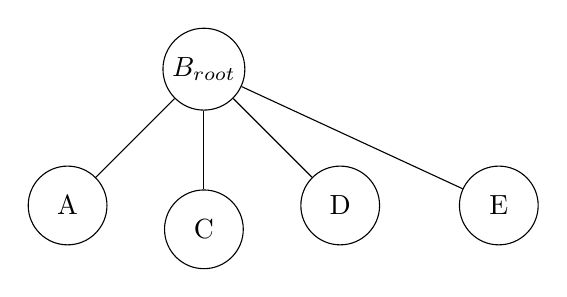
\begin{tikzpicture}
  [every node/.style={circle, draw, minimum size=1cm, inner sep=2pt}]
  \node (B) {$B_{root}$};
  \node (A) [below left=of B] {A};
  \node (C) [below=of B] {C};
  \node (D) [below right=of B] {D};
  \node (E) [right=of D] {E};
  
  \draw (B) -- (A);
  \draw (B) -- (C);
  \draw (B) -- (D);
  \draw (B) -- (E);
\end{tikzpicture}
\end{center}
This structure satisfies the acyclic and tree properties, with \( B \) designated as the root node.

\subsection{Graph with No Cycles That is Not a Tree}
A forest (a set of disjoint trees) meets this criterion. For example, with nodes \( A, B, C, D, \) and \( E \), we could have two disjoint trees, such as \( A - B \), \( C - D \), and \(E\), which is a graph without cycles and that is not a single tree.

\begin{center}
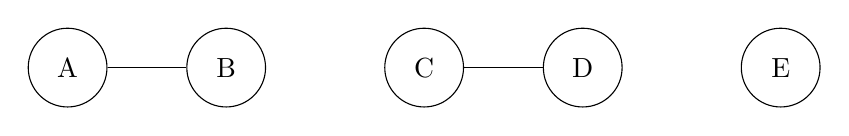
\begin{tikzpicture}
  [every node/.style={circle, draw, minimum size=1cm, inner sep=2pt}]
  \node (A) {A};
  \node (B) [right=of A] {B};
  \node (C) [right=1.5cm of B] {C};
  \node (D) [right=of C] {D};

  \node (E) [right= 1.5cm of D] {E};
  
  \draw (A) -- (B);
  \draw (C) -- (D);
  \draw (E);
\end{tikzpicture}
\end{center}

Alternatively we could use a directed graph with nodes \( A, B, C, D, \) and \( E \) and edges \( A \rightarrow B \), \( B \rightarrow C \), \( C \rightarrow D \), and \( D \rightarrow E \), which is acyclic but not a tree.
\begin{center}
    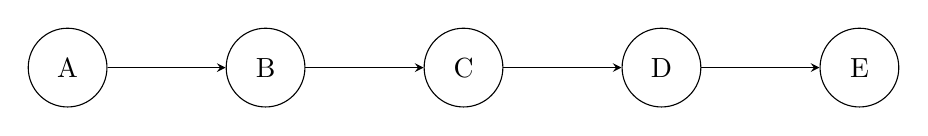
\begin{tikzpicture}[->, >=stealth, node distance=1.5cm, 
                        every node/.style={circle, draw, minimum size=1cm, inner sep=2pt}]
      
      % Nodes
      \node (A) {A};
      \node (B) [right=of A] {B};
      \node (C) [right=of B] {C};
      \node (D) [right=of C] {D};
      \node (E) [right=of D] {E};
      
      % Directed Edges
      \draw (A) -> (B);
      \draw (B) -> (C);
      \draw (C) -> (D);
      \draw (D) -> (E);
    
    \end{tikzpicture}
\end{center}

\subsection{Weighted Graph Where Every Path from \( A \) to \( E \) Has Weight 2}
Consider a graph with paths \( A - B - E \), \( A - D - E \), and \( A - C - E \), where each edge has a weight of 1. Both paths from \( A \) to \( E \) thus have a total weight of 2, satisfying the condition.

\begin{center}
    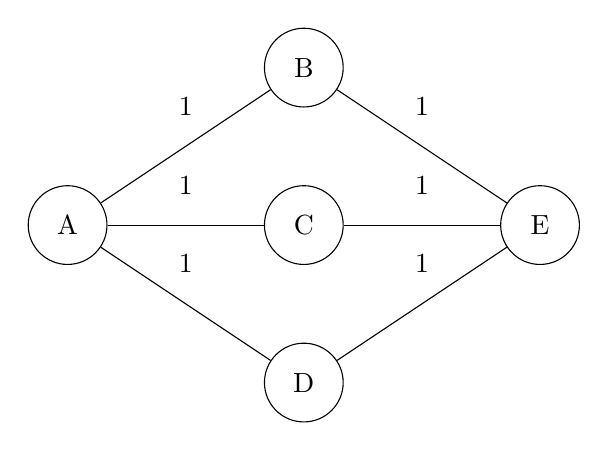
\begin{tikzpicture}
      % Set up nodes
      [every node/.style={circle,draw, minimum size=1cm, inner sep=2pt}]
      
      \node (A) at (0,2) {A};
      \node (B) at (3,4) {B};
      \node (C) at (3,2) {C};
      \node (D) at (3,0) {D};
      \node (E) at (6,2) {E};
      
      % Draw edges with weights
      \draw (A) -- node[draw=none, above] {1} (B);
      \draw (A) -- node[draw=none, above] {1} (C);
      \draw (A) -- node[draw=none, above] {1} (D);
      \draw (B) -- node[draw=none, above] {1} (E);
      \draw (C) -- node[draw=none, above] {1} (E);
      \draw (D) -- node[draw=none, above] {1} (E);

    \end{tikzpicture}
    \end{center}

\subsection{Rooted Tree with Minimal Number of Leafs}
To minimize the number of leaf nodes in a rooted tree of 5 nodes, we arrange the nodes in a straight line where each node connects to exactly one other, except the root. For example:
\begin{center}
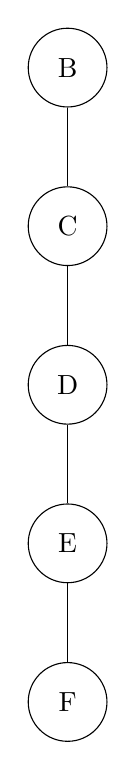
\begin{tikzpicture}
  [every node/.style={circle, draw, minimum size=1cm, inner sep=2pt}]
  \node (B) {B};
  \node (C) [below=of B] {C};
  \node (D) [below=of C] {D};
  \node (E) [below=of D] {E};
  \node (F) [below=of E] {F};
  
  \draw (B) -- (C) -- (D) -- (E) -- (F);
\end{tikzpicture}
\end{center}
This structure has only one leaf node \( F \), which minimizes the number of leaves.

\subsection{Strongly Connected Directed Graph with 5 Nodes with Minimal Edges}
To form a strongly connected directed graph with 5 nodes and the minimum number of edges, we create a directed cycle among the nodes: \( A \rightarrow B \rightarrow C \rightarrow D \rightarrow E \rightarrow A \). This configuration has exactly 5 edges, ensuring strong connectivity.

\begin{center}
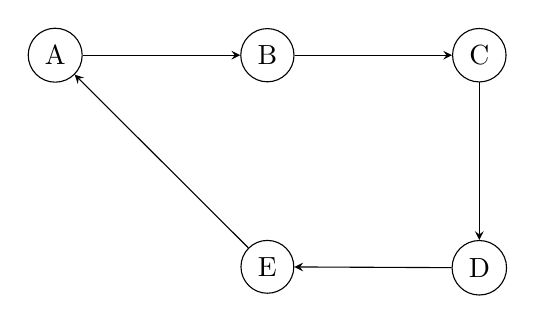
\begin{tikzpicture}[->, >=stealth, auto, node distance=2cm, every node/.style={circle, draw}]
  \node (A) {A};
  \node (B) [right=of A] {B};
  \node (C) [right=of B] {C};
  \node (D) [below=of C] {D};
  \node (E) [below=of B] {E};

  \draw (A) -- (B);
  \draw (B) -- (C);
  \draw (C) -- (D);
  \draw (D) -- (E);
  \draw (E) -- (A);
\end{tikzpicture}
\end{center}

\newpage

\section{Family Tree}

\subsection{Child of \( D \)}
The children of \( D \) is \( C \) and $E$.

\subsection{Parent of \( I \)}
The parent of \( I \) is \( H \).

\subsection{Sibling of \( D \)}
The sibling of \( D \) is \( A \).

\subsection{Ancestor of \( H \)}
The ancestors of \( H \) are \( I \), \( G \), and $F$, as are on the path from \( H \) to the root node \( F \).

\subsection{Descendent of \( B \)}
The descendents of \( B \) are all nodes below it in the tree: \( A, D, C, \) and \( E \).

\subsection{Neighbors of \( D \) or \( G \) Not Also Neighbors of \( B \)}
The neighbors of \( D \) are \( B \), $F$ and \( E \), and the neighbors of \( G \) are \( D \), $I$ and \( F \). Excluding neighbors of \( B \), which are $A$ and $D$, the nodes satisfying this condition are $E$, \( F \) and $I$.

\newpage

\section{Graph Representation}

\subsection{Adjacency List Representation of \( G_{undirected} \)}
The adjacency list of \( G_{undirected} \) is:
\[
\begin{aligned}
    1 & : 2, 3 \\
    2 & : 1, 3 \\
    3 & : 1, 2, 4 \\
    4 & : 3 \\
\end{aligned}
\]

\subsection{Adjacency Matrix Representation of \( G_{undirected} \)}
The adjacency matrix for \( G_{undirected} \) is:
\[
  \begin{bNiceMatrix}[first-row,first-col]
        & 1   & 2   & 3   & 4 \\
    1   & 0   & 1   & 1   & 0 \\
    2   & 1   & 0   & 1   & 0 \\
    3   & 1   & 1   & 0   & 1 \\
    4   & 0   & 0   & 1   & 0 \\
  \end{bNiceMatrix}
\]

\subsection{Adjacency List Representation of \( G_{directed} \)}
The adjacency list for \( G_{directed} \) is:
\[
\begin{aligned}
    1 & : 2, 3 \\ 
    2 & : \text{(none)} \\ 
    3 & : 2, 4 \\ 
    4 & : 3 \\ 
\end{aligned}
\]

\subsection{Adjacency Matrix Representation of \( G_{directed} \)}
The adjacency matrix for \( G_{directed} \) is:
\[
  \begin{bNiceMatrix}[first-row,first-col]
      & 1 & 2 & 3 & 4 \\
    1 & 0 & 1 & 1 & 0 \\
    2 & 0 & 0 & 0 & 0 \\
    3 & 0 & 1 & 0 & 1 \\
    4 & 0 & 0 & 1 & 0 \\
  \end{bNiceMatrix}
\]

\newpage

\section{BFS / DFS Traversals}
Redrawing the graph to better visualize the nodes and their connections:
\begin{center}
  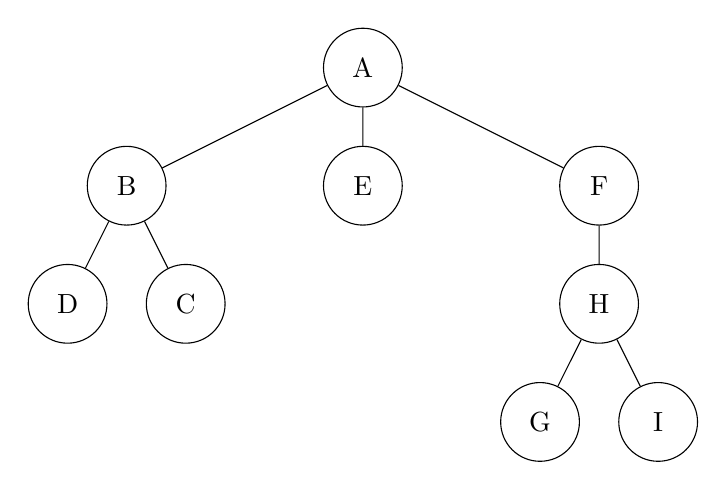
\begin{tikzpicture}[
    every node/.style={circle, draw, minimum size=1cm, inner sep=0pt},
    level 1/.style={sibling distance=3cm},
    level 2/.style={sibling distance=1.5cm}
  ]

  % Root node
  \node {A}
      % Level 1
      child {node {B}
          % Level 2 under B
          child {node {D}}
          child {node {C}}
      }
      child {node {E}}
      child {node {F}
        % Level 2 under F
        child {node {H}
          % Level 3 under H
          child {node {G}}
          child {node {I}}
          }
      };

  \end{tikzpicture}
\end{center}

\subsection{Breadth First Search (BFS) starting at Node A}

In Breadth First Search, we explore nodes level by level from the starting node.

\begin{enumerate}
    \item Start at node \( A \).
    \item Visit the children of \( A \): \( B \), \( E \), \( F \).
    \item Visit the children of \( B \): \( D \), \( C \).
    \item Visit the children of \( F \): \( H \).
    \item Visit the children of \( H \): \( G \), \( I \).
\end{enumerate}

\textbf{Order:} \( A, B, E, F, D, C, H, G, I \)

\subsection{Depth First Search (DFS) starting at Node A}

In Depth First Search, we explore as far down each branch as possible before backtracking.

\begin{enumerate}
    \item Start at node \( A \).
    \item Move to \( B \).
    \item Move to \( D \).
    \item Backtrack to \( B \), then move to \( C \).
    \item Backtrack to \( A \), then move to \( E \).
    \item Backtrack to \( A \), then move to \( F \).
    \item Move to \( H \).
    \item Move to \( G \).
    \item Backtrack to \( H \), then move to \( I \).
\end{enumerate}

\textbf{Order:} \( A, B, D, C, E, F, H, G, I \)

\subsection{Breadth First Search (BFS) starting at Node F}

Starting from \( F \) and using BFS:

\begin{enumerate}
    \item Start at node \( F \).
    \item Visit the children of \( F \): \( H \).
    \item Visit the children of \( H \): \( G \), \( I \).
\end{enumerate}

\textbf{Order:} \( F, H, G, I \)

\subsection{Depth First Search (DFS) starting at Node F}

Starting from \( F \) and using DFS:

\begin{enumerate}
    \item Start at node \( F \).
    \item Move to \( H \).
    \item Move to \( G \).
    \item Backtrack to \( H \), then move to \( I \).
\end{enumerate}

\textbf{Order:} \( F, H, G, I \)
\newpage

\section{Shortest Path (Dijkstra's Algorithm)}

Using Dijkstra's algorithm, we compute the shortest path from \( A \) to \( G \). Below is the table showing the path weights and predecessors for each node.

\begin{table}[h]
  \centering
  \label{}
  \begin{tabular}{|c|c|c|c|c|c|c|c|c|}
  \hline
  iteration & node visited & A & B & C & D & E & F & G\\ \hline
  0 & A & start:0 & A:5 & A:5 & none & none & none & none\\ \hline
  1 & B & start:0 & A:5 & A:5 & B:14 & B:7 & none & none\\ \hline
  2 & C & start:0 & A:5 & A:5 & C:6 & B:7 & C:14 & none\\ \hline
  3 & D & start:0 & A:5 & A:5 & C:6 & B:7 & D:9 & none\\ \hline
  4 & E & start:0 & A:5 & A:5 & C:6 & B:7 & D:9 & E:15\\ \hline
  5 & F & start:0 & A:5 & A:5 & C:6 & B:7 & D:9 & F:13\\ \hline
  \end{tabular}
\end{table}
Now by backtracking from G to A. 
\[
G \rightarrow F \rightarrow D \rightarrow C \rightarrow A
\]
Thus, shortest path from \( A \) to \( G \) is:
\[A \rightarrow C \rightarrow D \rightarrow F \rightarrow G \text{, with a total weight of 13.}\]

\newpage

\section{Extra Credit: Airline Connectivity}

Given a graph representing flights among cities, if every pair of cities is connected by exactly one airline, there exists at least one airline that can connect any two cities via a sequence of flights, thus forming a connected graph for that airline.

\end{document}


\end{document}
